\section{Model Architecture}


The basic architecture of \modelname~is similar to Llama 3~\cite{grattafiori2024llama}. It has 135 billion parameters with a hidden dimension of 12,288, a SwiGLU~\cite{shazeer2020glu} feed-forward network (FFN) intermediate size of 28,672, and 94 layers. The attention blocks in \modelname~leverage Group Query Attention (GQA) to reduce KV-cache size by incorporating 96 query heads and 8 KV heads.

There are two crucial differences to address the fundamental challenges of training stability and convergence in large dense LLMs. We propose Depth-Scaled Sandwich-Norm to replace the layer normalization and TinyInit for parameter initialization. By integrating these techniques, \modelname~achieves substantial improvements over previous dense models.


\subsection{Depth-Scaled Sandwich-Norm}

Large-scale dense models typically adopt deeper architectures \cite{dubey2024llama}, although MoE models usually scale in width \cite{deepseekv3}. However, increased depth introduces greater challenges in maintaining training stability. 
Given the prohibitive cost of pre-training, stable training of large dense LLMs becomes paramount.
Pre-Layer Normalization (Pre-LN) has been found to make back-propagation more efficient for deep Transformers \cite{wang2019learning-deep}, leading to its widespread adoption in Transformer-based large language model (LLM) architectures \cite{dubey2024llama,bai2023qwen,deepseekv3}.



However, in models employing the pre-LN structure, the fluctuating output scale of each sub-layer can easily lead to training instability \cite{takase2024spikemore}.
To address this issue, sandwich-norm \cite{NEURIPS2021_CogView} applies an layer normalization to each sub-layer's output prior to the residual connection. While the sandwich-norm maintains the scale stability of individual sub-layer outputs, the progressive accumulation of output norms via residual connections across multiple layers may nevertheless lead to training instability.

To mitigate this, we present the depth-scaled sandwich norm, which integrates the sandwich norm with a depth-scaled initialization scheme. The layer normalization regulates layer-wise output magnitudes through trainable gamma parameters, which are initialized with values scaled proportionally to the inverse of network depth. Figure ~\ref{fig:sandwich_arch} illustrates the differences between the depth-scaled sandwich-norm and pre-norm architectures. The formula of depth-scaled sandwich-norm is


\begin{equation} \label{eq:sandwich}
\begin{aligned}
    \mathbf{h} &\leftarrow \mathbf{h} + {\text{Norm}}({\gamma_{\text{attn}}}, \text{ATTN}(\text{Norm}(\mathbf{h}))), \quad  \gamma_{\text{attn}} = \frac{c_{\text{attn}}}{\sqrt{L}},\\ 
    \mathbf{h} &\leftarrow \mathbf{h} + {\text{Norm}}({\gamma_{\text{mlp}}}, \text{MLP}(\text{Norm}(\mathbf{h}))), \quad \gamma_{\text{mlp}} = \frac{c_{\text{mlp}}}{\sqrt{L}}, \\
\end{aligned}
\end{equation}



where $L$ is the number of layers, $c_{\text{attn}}$ and $c_{\text{mlp}}$ are set as the initial output standard deviations of the attention layer and feed-forward network (FFN) layer, respectively. For \modelname, we set $c_{\text{attn}}$ to 0.283 and $c_{\text{mlp}} $ to 0.432 .


\begin{figure}[htbp]
    \centering
    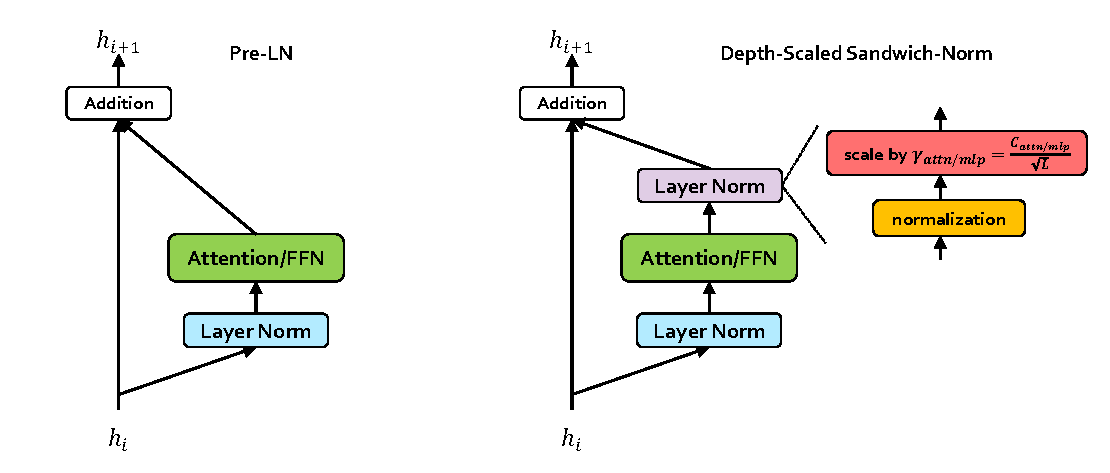
\includegraphics[width=0.8\textwidth]{fig/sandwich_arch.pdf}
    \caption{Structure comparison between Pre-Layer Norm (Pre-LN) and Depth-Scaled Sandwich-Norm (DSSN). DSSN applies normalization layers to both before and after the attention and FFN block, while Pre-LN only utilizes one normalization layer. DSSN also employs a depth-scaled initialization schema, which is not in the original sandwich norm.
    }
    \label{fig:sandwich_arch}
\end{figure}

\subsection{Model Initialization} \label{sec:tinyinit}

Existing works \cite{nguyen2019transformers} observe that model initialization plays a crucial role in training stability and performance. 
Transformer-based LLMs widely adopt small initialization\cite{nguyen2019transformers}, which initialze all the weight with a normal distribution of standard deviation  $\sqrt{\frac{2}{5d}}$, where $ d $ is the hidden dimension.
It's also common practice to scale the weights of residual layers at initialization by a factor of $ 1 / \sqrt{L}$ \cite{radford2019language}, where $ L $ is the number of
 layers. 



Our findings suggest that scaling initialization by both model depth and width, using $ \sqrt{\frac{1}{2dL}}$, leads to faster loss convergence and improved performance on downstream tasks. We call this initialization method TinyInit.
We hypothesize that TinyInit achieves more consistent parameter scales across the model, which may facilitate optimization and convergence. 

Research \cite{takase2024spikemore} indicates that embedding layers require different initialization strategies compared to other layers.
Specifically, maintaining the standard deviation of embedding weights close to 1 may enhance training stability. 
Our experimental results indicate that initializing with a standard deviation of 0.5 achieves good model performance.



\subsection{Tokenizer}\label{section:tokenizer}
The design of the tokenizer significantly impacts model performance. An optimal vocabulary balances domain coverage (handling diverse tasks such as text, math, and code) with efficiency (encoding data with fewer tokens). Common methods use Byte-Pair Encoding (BPE)~\cite{shibata1999byte} and SentencePiece~\cite{kudo-richardson-2018-sentencepiece} build vocabularies by directly computing word frequencies across the entire training dataset. However, this approach suffers from domain imbalance, as common domains such as general text dominate the vocabulary, while specialized domains such as math and code remain underrepresented due to their limited data volume.


\modelname~adopts a domain-aware vocabulary strategy. We perform independent frequency analyses across multiple domains including general Chinese, general English, code, and mathematics, generating distinct domain-specific vocabularies. These vocabularies are then merged and de-duplicated to form a unified vocabulary of 153,376 unique tokens, maintaining balanced representation across domains while preserving overall compression efficiency. Table~\ref{tab:vocab_distribution} summarizes the detailed token distribution across different domains.
\begin{table}[htbp]
\centering
\caption{Token distribution in the unified vocabulary of \modelname.}
\label{tab:vocab_distribution}
\small
\begin{tabular}{lrr}
\toprule
\textbf{Domain} & \textbf{Number of Tokens} & \textbf{Percentage (\%)} \\
\midrule
English & 68,017 & 44.35 \\
Chinese & 41,053 & 26.77 \\
Other & 30,573 & 19.93 \\
Latin-based languages & 4,507 & 2.94 \\
Arabic & 2,755 & 1.80 \\
Korean & 2,733 & 1.78 \\
Mathematics & 2,139 & 1.39 \\
Japanese & 1,599 & 1.04 \\

\midrule
\textbf{Total} & \textbf{153,376} & \textbf{100.00} \\
\bottomrule
\end{tabular}
\end{table}
